\documentclass[12pt,letterpaper]{article}
\usepackage[utf8]{inputenc}
\usepackage[T1]{fontenc}
\usepackage{amsmath}
\usepackage{amsfonts}
\usepackage{amssymb}
\usepackage{graphicx}
\title{An Example Paper Generated with GNU Make}
\author{Joseph T. Ornstein}
\date{June 26, 2020}

\begin{document}
	
	\maketitle
	
	\section{This is my first section}
	
	
	Some filler text and then a table.
	
	% latex table generated in R 4.0.2 by xtable 1.8-4 package
% Mon Aug 17 11:08:31 2020
\begin{table}[ht]
\centering
\begin{tabular}{rrr}
  \hline
 & y & x \\ 
  \hline
1 & 0.44 & 0.22 \\ 
  2 & 0.20 & 0.35 \\ 
  3 & 0.57 & 0.02 \\ 
  4 & 0.20 & 0.74 \\ 
  5 & 0.06 & 0.32 \\ 
  6 & 0.73 & 0.48 \\ 
  7 & 0.43 & 0.45 \\ 
  8 & 0.69 & 0.31 \\ 
  9 & 0.16 & 0.82 \\ 
  10 & 0.37 & 0.49 \\ 
   \hline
\end{tabular}
\end{table}

	
	And another table.
	
	% latex table generated in R 4.0.2 by xtable 1.8-4 package
% Mon Aug 17 11:08:31 2020
\begin{table}[ht]
\centering
\begin{tabular}{rrr}
  \hline
 & mean\_x & mean\_y \\ 
  \hline
1 & 0.48 & 0.48 \\ 
   \hline
\end{tabular}
\end{table}
	
	
	Now here's a figure.
	
	\begin{figure}
		\caption{A caption here...}
		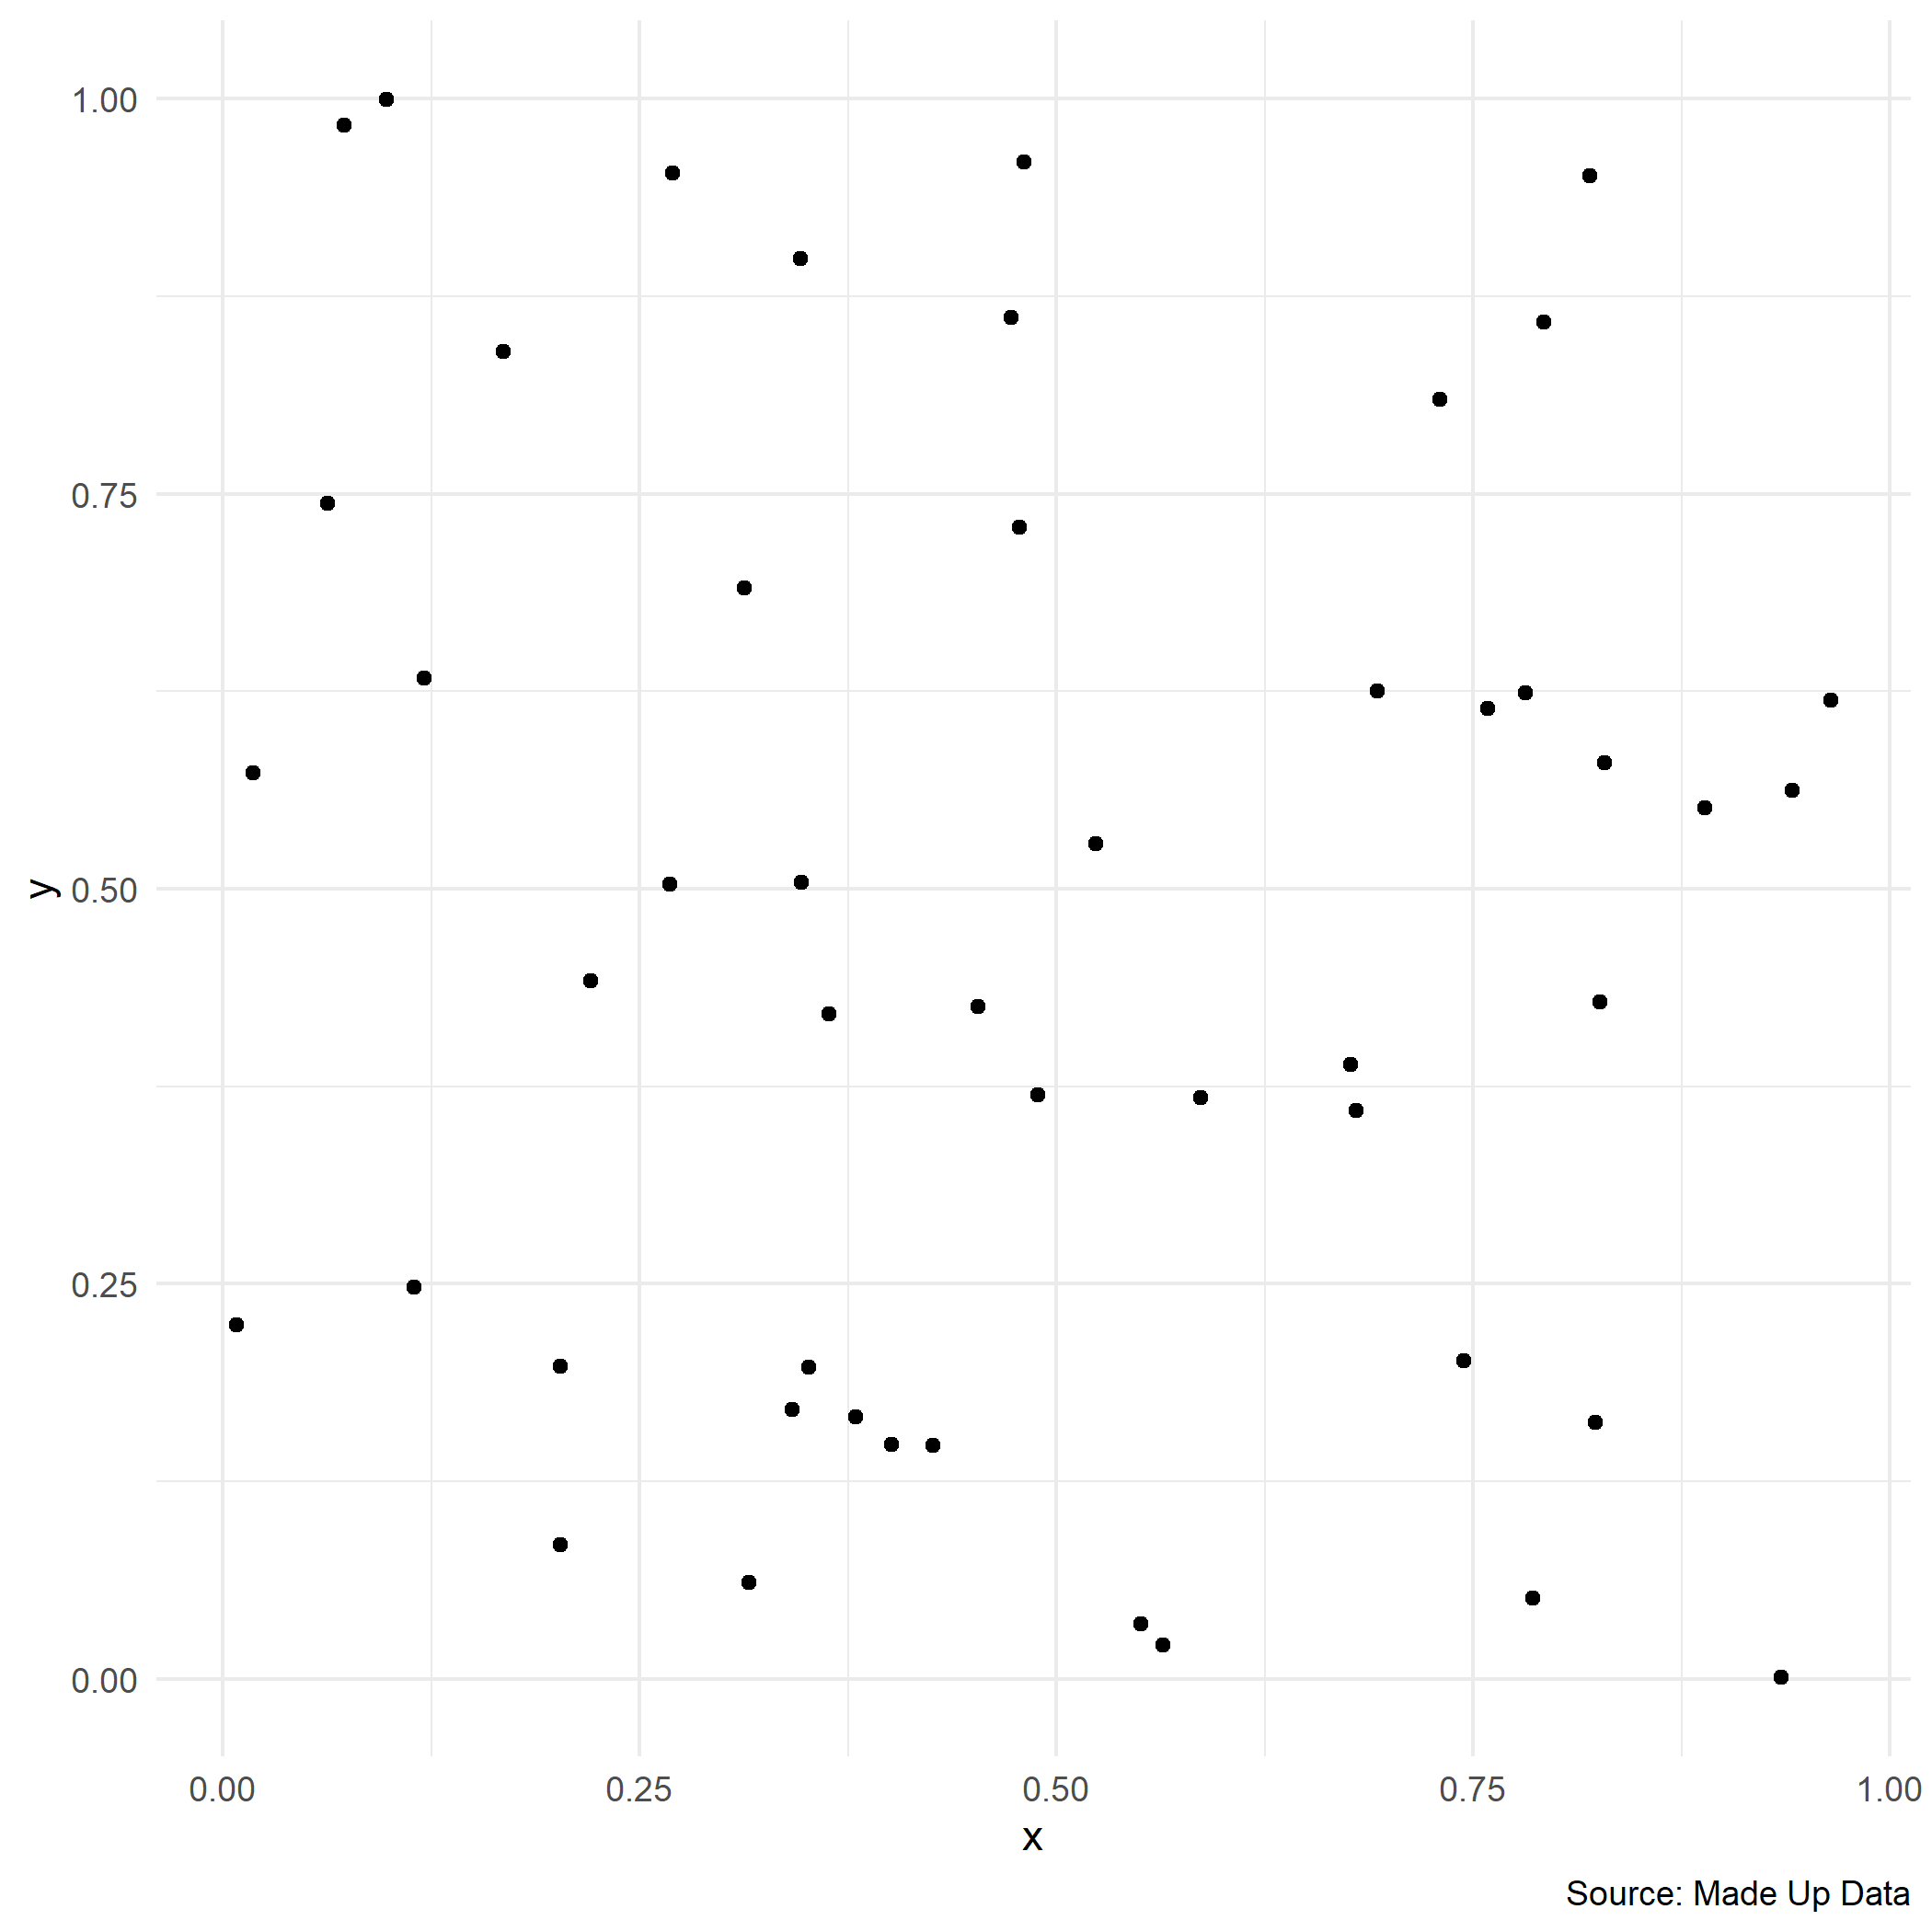
\includegraphics[width=0.9\textwidth]{figures/fig1.png}
	\end{figure}
	
	
	
\end{document}